% !TEX TS-program = pdflatex
% !TEX encoding = UTF-8 Unicode

% This is a simple template for a LaTeX document using the "article" class.
% See "book", "report", "letter" for other types of document.

\documentclass[11pt]{article} % use larger type; default would be 10pt

\usepackage[utf8]{inputenc} % set input encoding (not needed with XeLaTeX)

%%% Examples of Article customizations
% These packages are optional, depending whether you want the features they provide.
% See the LaTeX Companion or other references for full information.

%%% PAGE DIMENSIONS
\usepackage{geometry} % to change the page dimensions
\geometry{a4paper} % or letterpaper (US) or a5paper or....
% \geometry{margin=2in} % for example, change the margins to 2 inches all round
% \geometry{landscape} % set up the page for landscape
%   read geometry.pdf for detailed page layout information

\usepackage{graphicx} % support the \includegraphics command and options
% \usepackage[parfill]{parskip} % Activate to begin paragraphs with an empty line rather than an indent

%%% PACKAGES
\usepackage{booktabs} % for much better looking tables
\usepackage{array} % for better arrays (eg matrices) in maths
\usepackage{paralist} % very flexible & customisable lists (eg. enumerate/itemize, etc.)
\usepackage{verbatim} % adds environment for commenting out blocks of text & for better verbatim
\usepackage{subfig} % make it possible to include more than one captioned figure/table in a single float
\usepackage{blindtext}


%%% END Article customizations

%%% The "real" document content comes below...

\title{Brief Article}
\author{The Author}
%\date{} % Activate to display a given date or no date (if empty),
         % otherwise the current date is printed 

\begin{document}
\maketitle

\section{First section}

Your text goes here.

\subsection{A subsection}

More text.

\section{An image}
\begin{figure}[ht]
  \caption{A picture of a gull.}
  \centering
    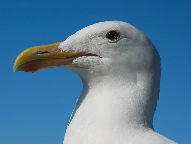
\includegraphics[width=0.5\textwidth]{gull}
\end{figure}

\begin{figure}[ht]
  \centering
    \reflectbox{%
      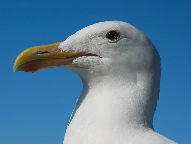
\includegraphics[width=0.5\textwidth]{gull}}
  \caption{A picture of the same gull
           looking the other way!}
\end{figure}

\blindtext

\section{A table}

\begin{table}[ht]
  \centering
    \begin{tabular}{| l c r |}
    \hline
    1 & 2 & 3 \\
    4 & 5 & 6 \\
    7 & 8 & 9 \\
    \hline
    \end{tabular}
  \caption{A simple table}
\end{table}

Notice how the tables and figures
have independent counters.

\section{Making lists. Itemize vs Enumerate.}
\subsection{A bulleted (unordered) list}

\begin{itemize}
  \item The individual entries are indicated with a black dot, a so-called bullet.
  \item The text in the entries may be of any length.
\end{itemize}

\subsection{A numbered (ordered) list}

% Guario: This is a comment

\begin{enumerate}
  \item This is the first entry in our list.
  \item The list numbers increase with each entry we add.
\end{enumerate}

\end{document}

